% Number 110
% CAPM Motionmap
% Car speeds up, slows down: MC pick motion map
% MIT Physics for Teachers LON-CAPA

% Watermark
\AddToShipoutPicture*{\BackgroundPic}

\addtocounter {ProbNum} {1}

\begin{floatingfigure}[r]{.3\textwidth}
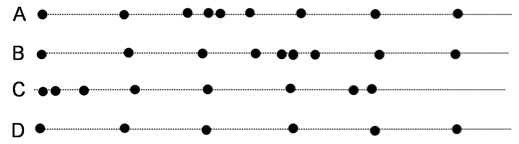
\includegraphics[scale=.4]{/Users/jgates/desktop/latex/pics/Motionmap1.png}
\end{floatingfigure}
 
{\bf \Large{\arabic{ProbNum}}} Driving a car in the positive x direction at a speed of 60 mph, Mary tests her brakes by coming to a complete stop in 4 seconds. Then she accelerates to her original speed of 60 mph in 8 seconds. A motion diagram is created by illuminating her car with a strobe at 2 second intervals. 

 \bigskip

\indent Which of the following best represents the correct diagram? Mary�s car is represented by a dot.   
 

\vfill

\newpage
